\begin{figure}[!htb]
	\centering
	\begin{subfigure}{0.45\textwidth}
		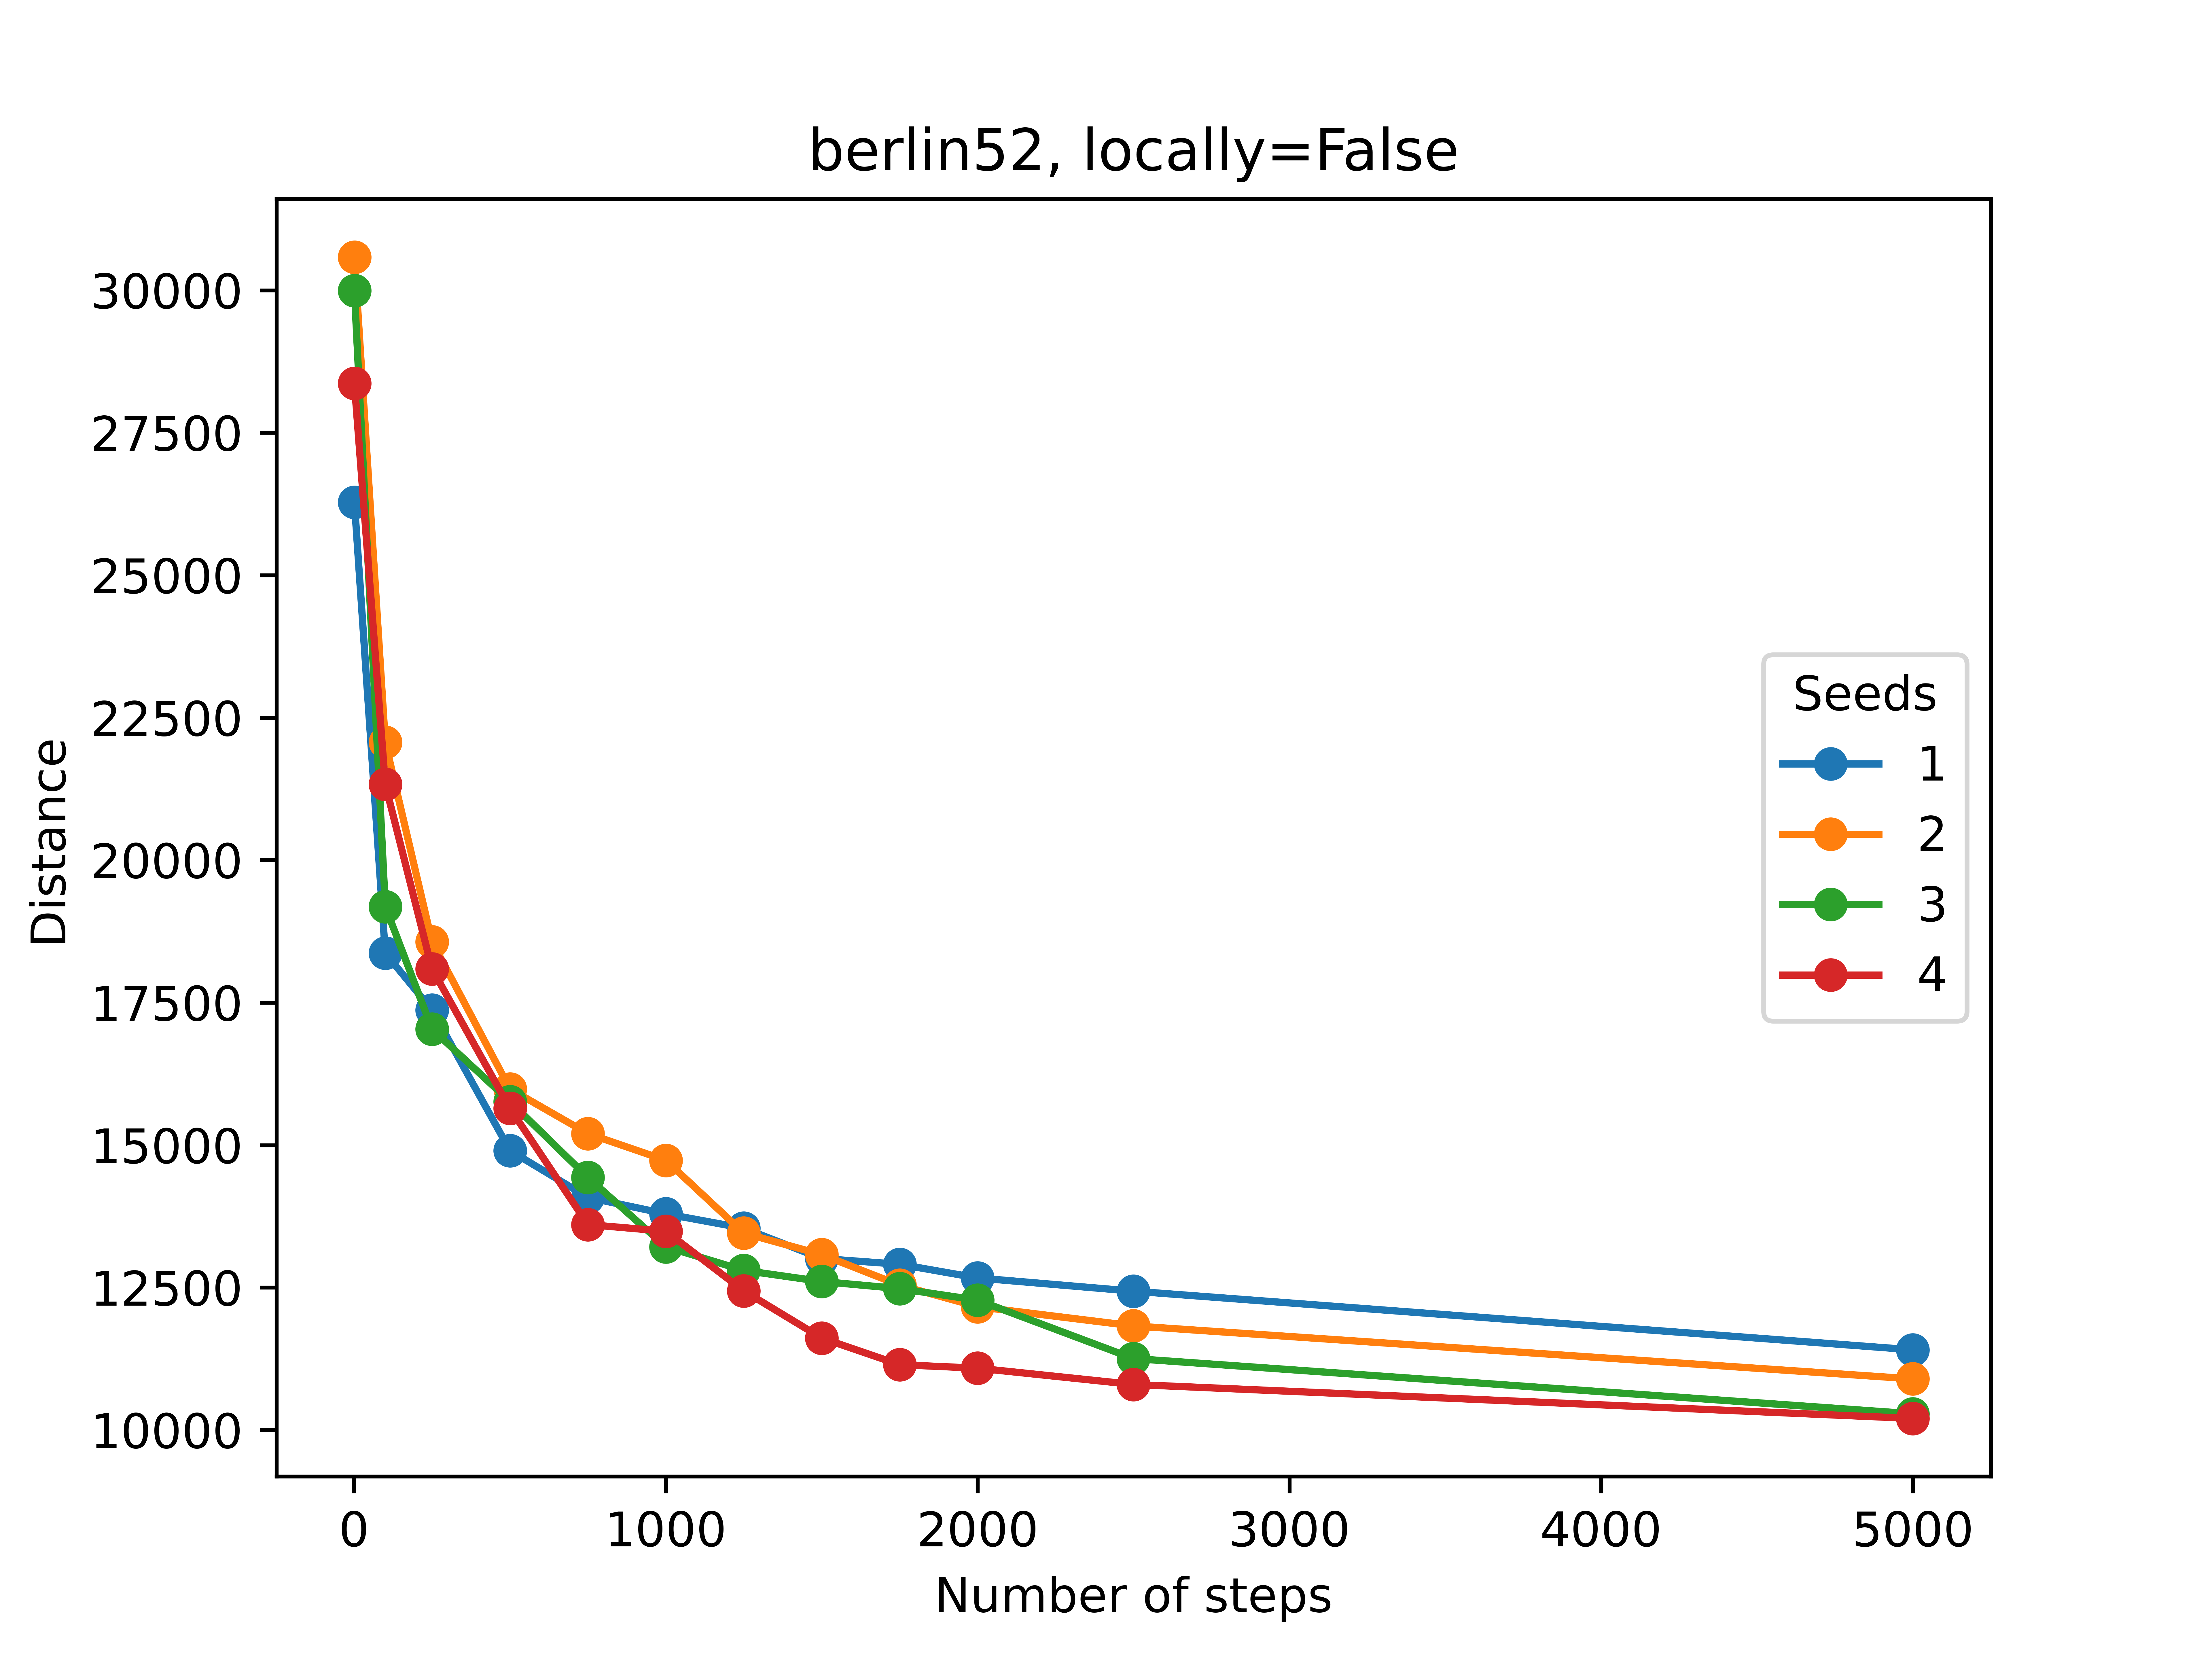
\includegraphics[width=\textwidth]{img/berlin52_seeds_locally=False}
		\subcaption{Random candidates.}
	\end{subfigure}
	\begin{subfigure}{0.45\textwidth}
		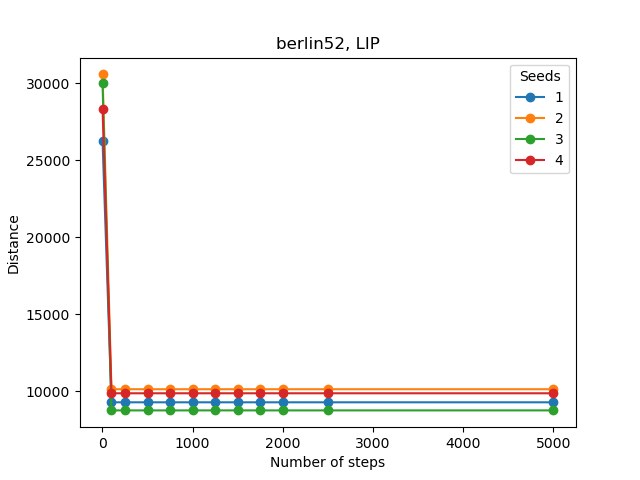
\includegraphics[width=\textwidth]{img/berlin52_seeds_locally=True}
		\subcaption{Locally-informed proposals.}
	\end{subfigure}
	\caption{Distances over number of steps for \textit{berlin52} dataset and different initial states.}
	\label{fig:berlin52_seeds}
\end{figure}
	
\begin{figure}[!htb]
	\centering
	\begin{subfigure}{0.45\textwidth}
		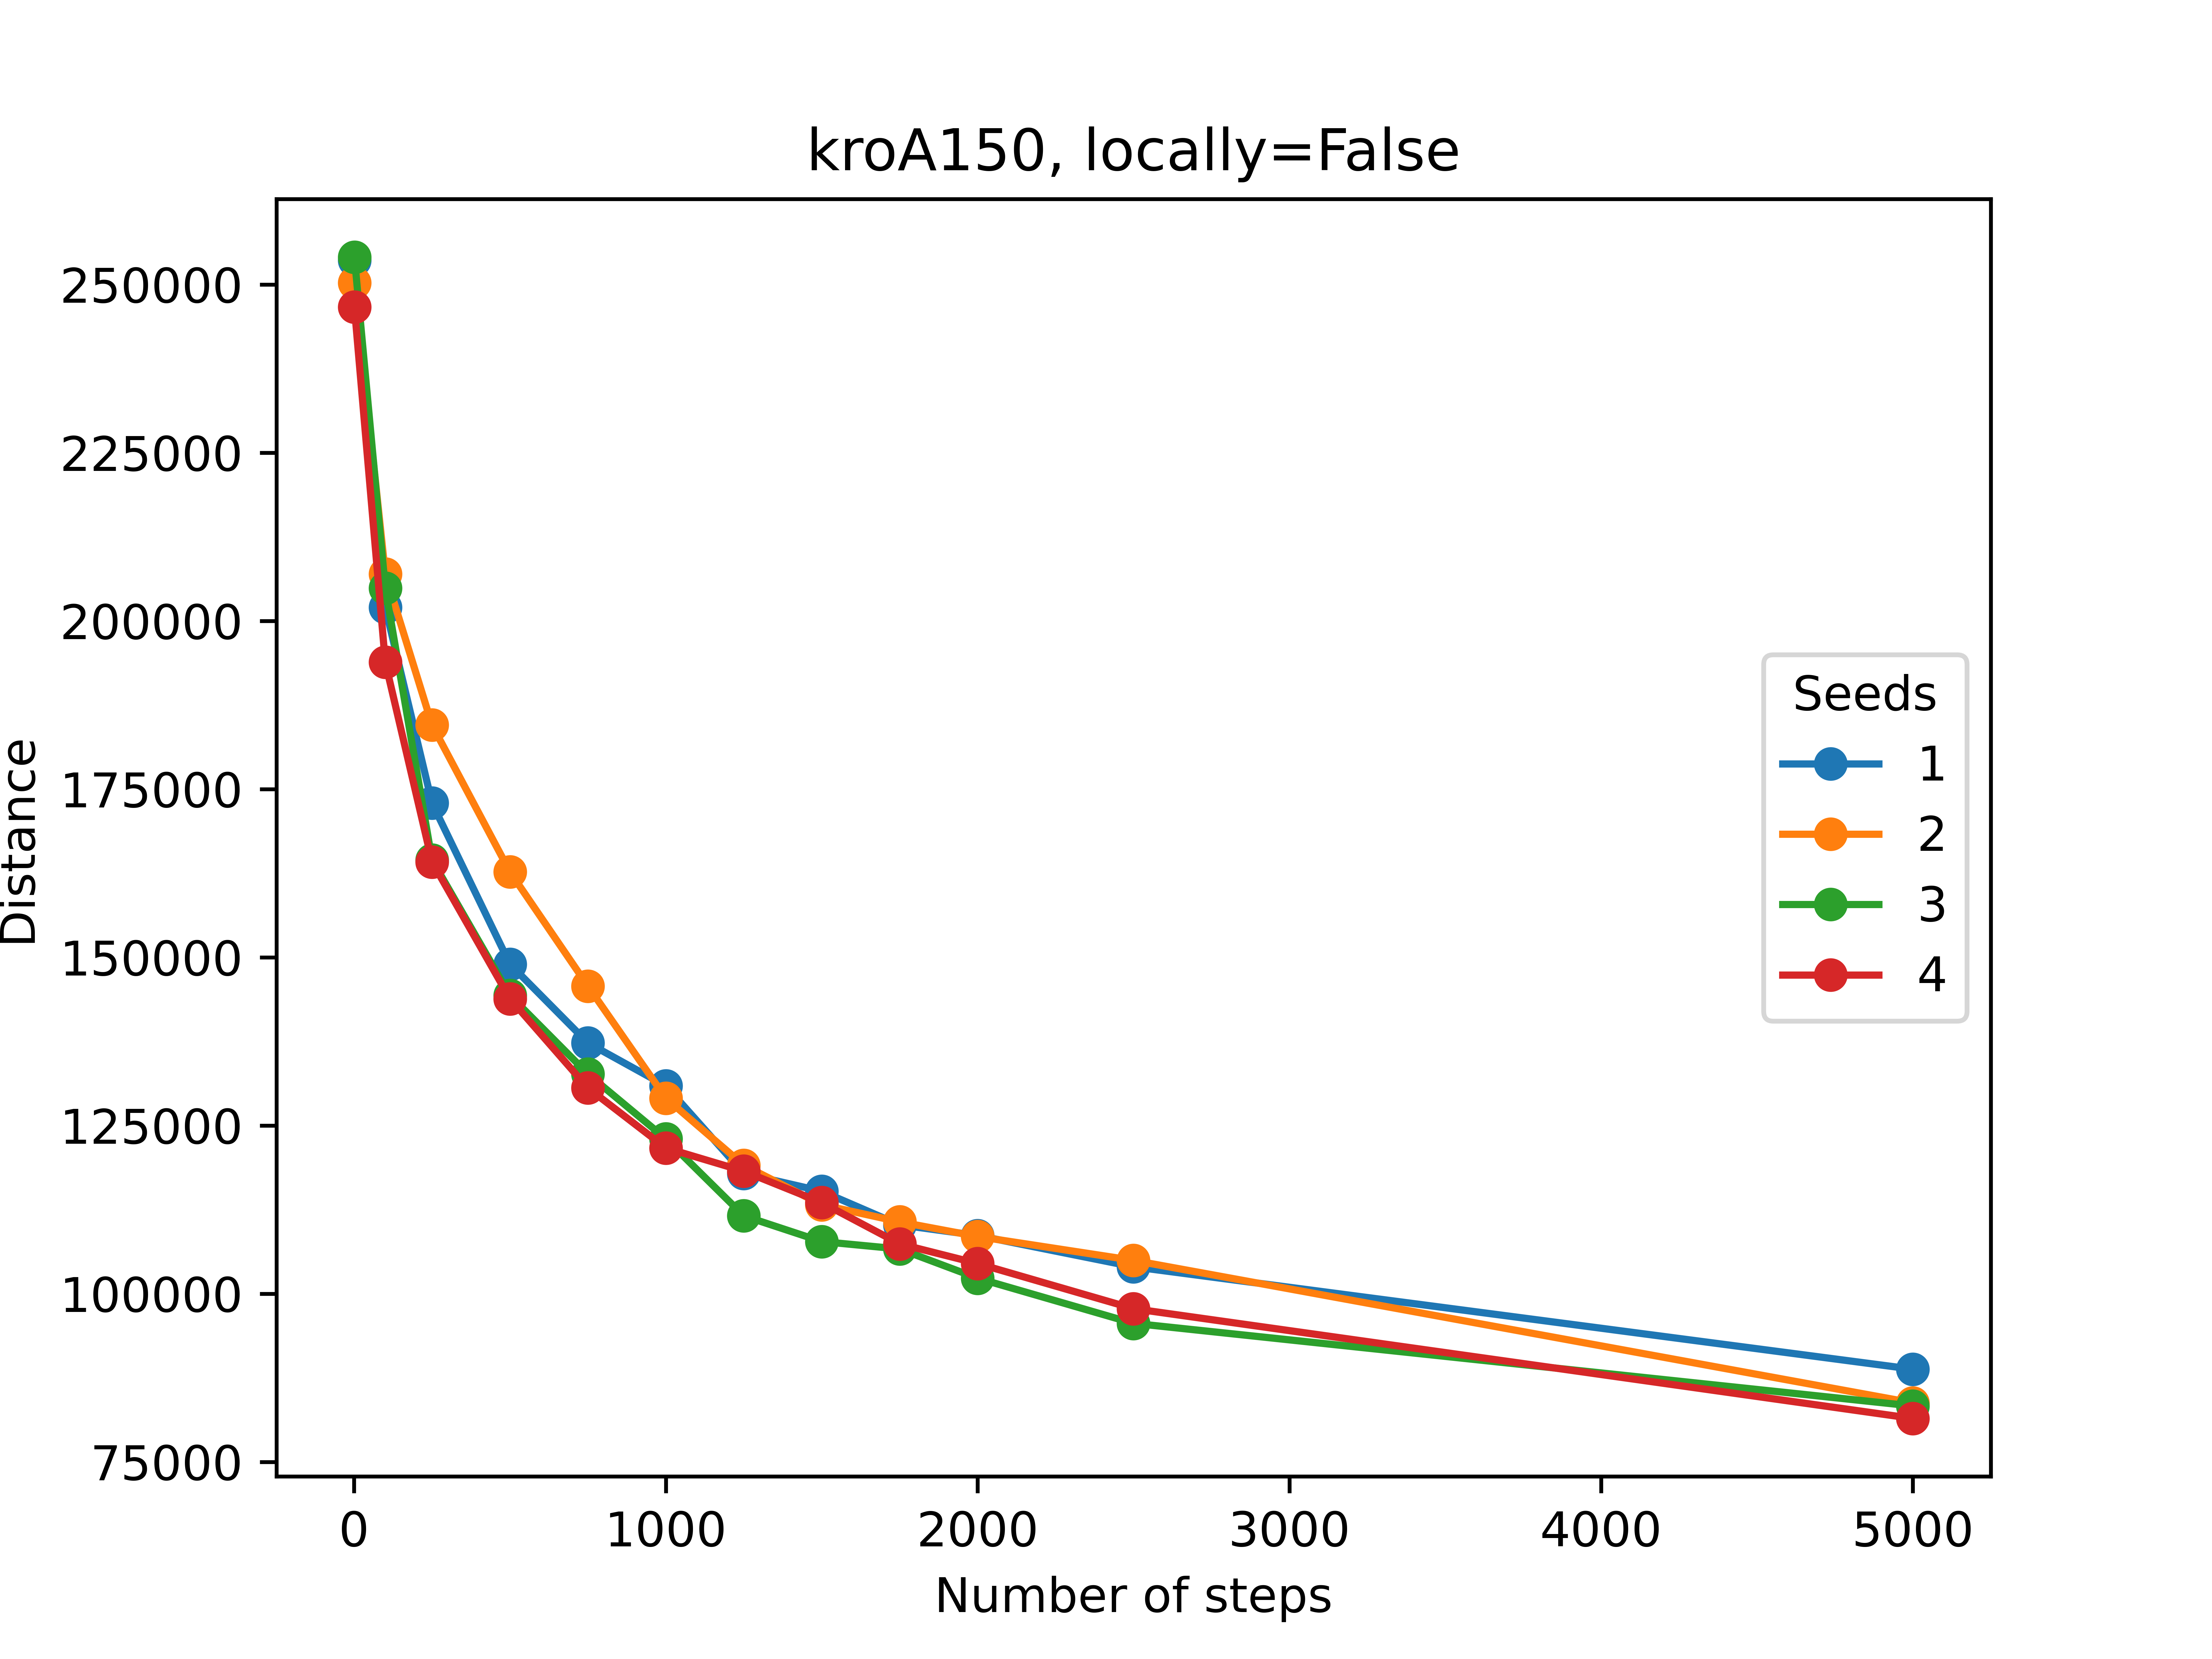
\includegraphics[width=\textwidth]{img/kroA150_seeds_locally=False}
		\subcaption{Random candidates.}
	\end{subfigure}
	\begin{subfigure}{0.45\textwidth}
		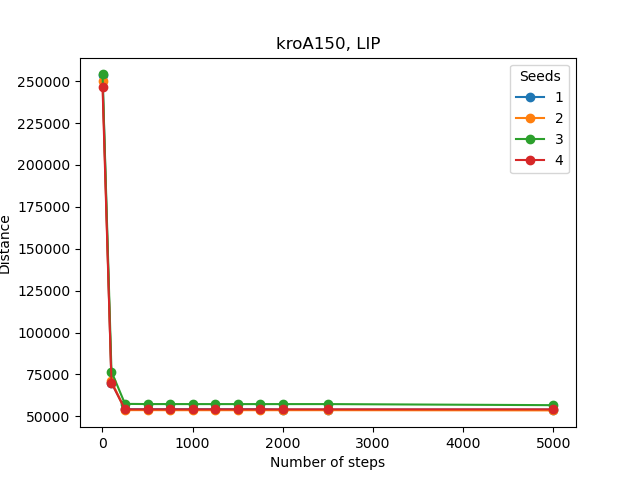
\includegraphics[width=\textwidth]{img/kroA150_seeds_locally=True}
		\subcaption{Locally-informed proposals.}
	\end{subfigure}
	\caption{Distances over number of steps for \textit{kroA150} dataset and different initial states.}
	\label{fig:kroA150_seeds}
\end{figure}